%\documentclass[document.tex]{subfiles}
%\begin{document}

%%{\section{The Purpose of the Project}\label{sec:Purpose}}
\subsection{Purpose of the project}
\edcomm{YS}{Added the ``AMMBR section'' based on comments from Dr. Kahl. He has verified the section, I'll follow up with a proof read and other section of this document}

Ampersand follows a \emph{rule based} design principle. Rules are integral to an organization
and these are based on some principles and guidelines set by the organization.
Ampersand uses an ECA ( Event - Condition - Action) approach to make sure all rules are satisfied. An ideal information infrastructure supports employees and other stakeholders to maintain the rules of the business. To maintain a rule means to prevent or correct all violations that might occur due to any external or internal factor.
 
 A large portion of the Ampersand system is already in place; the primary focus of this project was to
augment Ampersand with increased capabilities for automation. The module ``Automatically Fix Violations'' in Figure ~\ref{fig:EFAproject} represents the EFA project and where it fits in the current version of Ampersand.
Ampersand relies on the AMMBR \citep{Ampersand} algorithm to help fix these data violations. 
The role 
of AMMBR in Ampersand is to generate functions which can restore violations
in the generated prototype for the given information system. In AMMBR, human involvement is only limited 
to representing rules (in the ADL files). While the Ampersand software still 
remains in development phase, there is no way of checking the correctness of 
the AMMBR method at a low level. 

Previously, the ExecEngine was used to 
maintain these business rules. This required the author of the ADL file 
to write PHP code which operates on strings in order to tell Ampersand
how violations should be fixed. This required the author of the 
ADL file to know PHP and have knowledge of the internals of Ampersand,
essentially making information hiding impossible if one wanted to use
the Exec Engine. 
 
The EFA project, an extension to the Ampersand system, allows 
the user of Ampersand to generate a prototype for their information
system in which invariants are automatically maintained by code 
generated by EFA, which is derived from the specification given by the user.

The ECA rules, which act as an input to EFA, are translated into human-readable
SQL. This can later be viewed in the command line using the
\verb|``--print-eca-info''| flag.  The generated SQL queries allow the
correctness of AMMBR to be checked by running code generated by AMMBR on actual
databases. Therefore, EFA will be an essential tool for testing AMMBR.

\begin{figure}[!htb]
\begin{center}
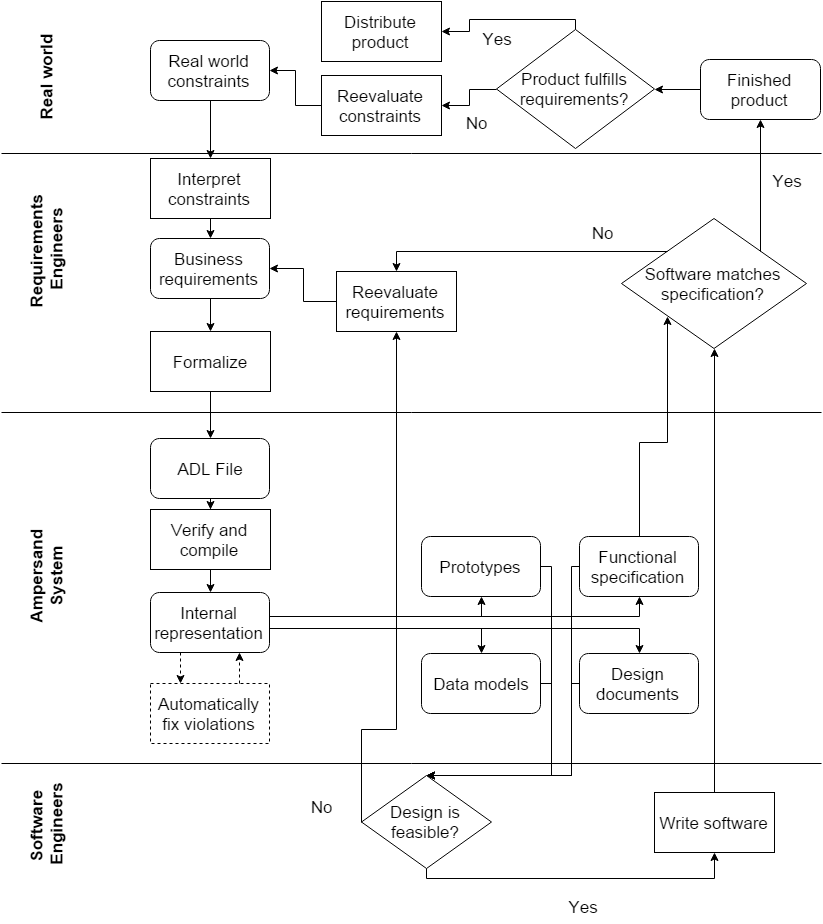
\includegraphics[width=\textwidth]{../figures/business_process}
\caption{Business process diagram representing EFA project represented as a dashed box}~\label{fig:EFAproject}
\end{center}
\end{figure}

 \subsection{The Stakeholders and the intended audience}\label{sec:Stakeholders}
The stake holders of Ampersand are:

\begin{description}
	\item[Ampersand Designers] Responsible for maintaining and developing Ampersand. The overall goal of Ampersand 
is to automate a large part of the software requirements and design process, and EFA fits this goal by greatly increasing
the amount of automation in the system, and therefore decreasing the burden on the user. Furthermore, EFA replaces the ExecEngine,
which allows more of Ampersand to be abstracted and simplifies the maintenance and design of the Ampersand code. 
	\item[The Customer] The end users of Ampersand will benefit from the EFA project. This will decreases the amount of time 
Ampersand users spend manually inserting PHP code to restore system invariants. The prototypes generated by Ampersand with the 
inclusion of EFA will be less error prone due fewer occurences of violations exposed to the user.
\end{description}

This document is intended to help introduce new Ampersand users to EFA 
(ECA rules for Ampersand) -- it provides a basic structure that allows 
individuals to quickly access the information they seek. It is also 
intended to describe the design, implementation, requirements and testing
of EFA for the Ampersand developers. 
